% ============================================================
%  CHAPTER 5 – Main Design Decisions
% ============================================================
\chapter{Design Decisions}
\label{ch:design-decisions}
This chapter discusses each of the major design decisions that have been made by each of the listed roles relative to their responsibilites. This chapter also discusses the alternatives to the chosen solutions and the reasons for the decisions made.

\section{EERI I:Subsystem: Drive Electronics}
\label{sec:eeri1-subsystem-drive-electronics}

The main power-electronic components were selected according to voltage and current requirments and switching
performance, thermal capacity compatibility with control circuitry and cost. Preference was given to components
that proivided sufficienty fault and trtansient headroom without exceeding the budget. The selected components 
were subsequently used during the low voltage test of the drive ciruitry.

\subsection{Bridge Rectifier}

In Table \ref{tab:eeri1-rectifiers} below the available bridge rectifiers for EEII are compared. 

\begin{table}[H]
    \centering
    \caption{Available bridge rectifiers for EEII I.}
    \label{tab:eeri1-rectifiers}

    \begin{tabular}{@{} l c c c c c @{}}
        \toprule
        \textbf{Component} &
        \shortstack{\textbf{Reverse Voltage}\\\textbf{Rating}} &
        \shortstack{\textbf{Average Current}\\\textbf{Rating}} &
        \shortstack{\textbf{Surge}\\\textbf{Current}} &
        \shortstack{\textbf{Thermal}\\\textbf{Resistance}} &
        \textbf{Selected} \\
        \midrule

        GBK25M & 1000 V & 25 A & 350 A & 0.6 $^\circ$C/W & \\

        GBJ1510 & 1000 V & 15 A & 240 A & 0.8 $^\circ$C/W & \checkmark \\

        \bottomrule
    \end{tabular}
\end{table}

Both rectifiers in Table \ref{tab:eeri1-rectifiers} provide a 1000V reverse-voltage rating, which gives a large margin above the 325VDC which 
is obtained from rectify in the 230VAC mains. The GBK25M porvides a higher 25A average current rating and 
350A surge current rating, whereas the GBJ1510 provides a 15A average and 240A surege current rating.

The GJB1510 was selected because its 15A average currnet rating is already well above the nominal current 
rating of the 180 W motor. The extra current capability of the GBK25M would therefore provide no additional
benefit during normal operation. The GBJ1510 still provides the necessary 1000V blocking capacity and 240A 
surge current rating is suffiecient for the application. The datasheet specifies that the rectifier current 
rating should be derated by 20 \% when supplying a capacitive load such as the bulk capacitor. Even after
derating the current capability remains well above the expected operating requirement. 

\subsection{IGBT Selection}

In Table \ref{tab:eeri1-igbt-options} below the available IGBTs for EEII are compared. 

\begin{table}[H]
    \centering
    \caption{Available IGBT options for EEII I.}
    \label{tab:eeri1-igbt-options}

    \small
    \begin{tabular}{@{} l c c c c c c @{}}
        \toprule
        \textbf{Component} &
        \shortstack{\textbf{Voltage}\\\textbf{Rating}} &
        \shortstack{\textbf{Current Rating}\\\textbf{@ 100$^\circ$C}} &
        \shortstack{\textbf{Pulsed}\\\textbf{Current}} &
        \shortstack{\textbf{Thermal}\\\textbf{Resistance}} &
        \shortstack{\textbf{Total Gate}\\\textbf{Charge}} &
        \textbf{Selected} \\
        \midrule

        STGP7NC60HD & 600 V & 14 A & 50 A & 1.56 $^\circ$C/W & 35 nC & \\

        FGH75T65SHDT & 650 V & 75 A & 225 A & 0.33 $^\circ$C/W & 123 nC & \checkmark \\

        \bottomrule
    \end{tabular}
\end{table}

Both devices in Table \ref{tab:eeri1-igbt-options} are suitable for the inverter application and provide voltage ratings well above the  nominal DC
bus voltage.The STGP7NC60HD is rated for 600V and 14A at a case temperature of 100$^\circ$C, with a pulsed current
rating of 50A. The FGH75T65SHDT increases these ratings to 650V and 75A at 100$^\circ$C and 225A pulsed current. 
It also has a significantly lower thermal resistance of 0.33 $^\circ$C/W. 

The FGH75T65SHDT was selected mainly for its greater voltage, transient currnet and thermanl margins. 
Although the nominal motor currnet is much lower than eitgher IGBT's continuous current rating, inverter
faults such as shoot-throughh and a phase-to-phase short can produce currents far greater than the normal operating
current. The higher pulsed-current therfore provides additional robustness while the protection circuit detects
the fualt and disalbles the inverter. 

A disadvantage of the FGH75T65SHDT is a larger gate charge of 123 nC compared to the approximately 35 nC of the
STGP7NC60HD. This places a greater load on the gate drivers and can increase losses. This trade-off was accepted 
because the intended switching frequency is relatively low and low-voltage prototype testing confirmed that the 
selected IR2104 driver and IGBT combination could successfully switch the test DC bus.

\subsection{Optocoupler Selection}

In Table \ref{tab:eeri1-optocoupler-options} below the available optocouplers for EEII are compared. 

\begin{table}[H]
    \centering
    \caption{Available optocoupler options for EEII I.}
    \label{tab:eeri1-optocoupler-options}

    \small
    \begin{tabular}{@{} l c c c c @{}}
        \toprule
        \textbf{Component} &
        \shortstack{\textbf{Isolation}\\\textbf{Voltage}} &
        \shortstack{\textbf{Typical Response}\\\textbf{Time}} &
        \shortstack{\textbf{Current Transfer}\\\textbf{Ratio}} &
        \textbf{Selected} \\
        \midrule

        PC817 &
        5000 V RMS &
        \shortstack{$t_r \approx 4\,\mu$s\\$t_f \approx 3\,\mu$s} &
        50--600\% &
        \\

        4N25 &
        5300 V RMS &
        \shortstack{$t_{on} \approx 4\,\mu$s\\$t_{off} \approx 3\,\mu$s} &
        20\% min. &
        \checkmark \\

        \bottomrule
    \end{tabular}
\end{table}

Both devices in Table \ref{tab:eeri1-optocoupler-options} provide galvanic isolation well above the 
voltage present in the inverter. The PC817 provides approximately 5000V RMS isolation, while the 4N25 is
rated for 5300 V RMS input-to-output isolation. Their typical switching speeds are also similar: the PC817 
has typical rise and fall times of approximately 4 µs and 3 µs, while the 4N25 specifies typical turn-on and 
turn-off times of approximately 4 µs and 3 µs.

The 4N25 was selected because it provides the required galvanic isolation function, a slightly higher isolation
voltage, and was succesfully obtained and tested as part of the prototype drive circuit. The PC817 has a higher 
current-transfer ratio, so the 4n25 is not superior in every electrical parameter but that is not the primary selection
criterion because the optocoupler is used to transmit logic-level PWM information rather than a analogue signal.

\subsection{Gate Driver Selection}

The IR2104 was selected as the half-bridge gate-driver IC. One IR2104 controls the high- and low-side IGBTs of 
each inverter leg, resulting in three driver ICs for the complete three-phase inverter. The device supports a 
floating high-side voltage of up to 600 V and operates from a 10 V to 20 V gate-drive supply. It is also compatible
with 3.3 V and 5 V logic levels.

An important reason for selecting the IR2104 is its integrated cross-conduction prevention and approximately 
520 ns internal dead time. These functions reduce the probability of simultaneous high- and low-side conduction 
within an inverter leg. The shutdown input can additionally disable both outputs, allowing the hardware protection
circuit to inhibit the inverter following an overcurrent fault.

\section{EERI II: Subsystem: Magnetic Load Attachment}
\label{sec:eeri2-subsystem-magnetic-load-attachment}
The design of the EERI II magnetic load attachment subsystem had the following to conceder:
the physical configuration and conection of the electromagnet,
the solid state switching and flyback clamp,
and the current sensing and analog conditioning.
 
\subsection{Electromagnet Configuration and Core Geometry}
\label{subsec:eeri2-dec-electromagnet}
Requirement DR3 strictly prohibits the use of complete COTS electromagnets,
while permitting COTS cores.
To safely hoist a 20\,kg steel plate ($196.2\,\text{N}$), the topology and magnetic circuit reluctance were evaluated across three configurations in Table~\ref{tab:eeri2-magnet-tradeoff}.

\begin{table}[H]
    \centering
    \small
    \caption{Trade-off evaluation of electromagnet configurations.}
    \label{tab:eeri2-magnet-tradeoff}
    \begin{tabularx}{\textwidth}{@{} >{\raggedright\arraybackslash}X c *{4}{c} c c @{}}
        \toprule
        \textbf{Configuration} & \textbf{DR3 Ok} & \textbf{Stability} & \textbf{Reluctance} & \textbf{Manufacture} & \textbf{Thermal} & \textbf{Score} & \textbf{Selected} \\
        \textit{Criteria weighting} & \textit{0.25} & \textit{0.25} & \textit{0.20} & \textit{0.15} & \textit{0.15} & \textit{(1--5)} & \\
        \midrule
        Single central pot core     & 2 & 2 & 4 & 4 & 3 & 2.85 & \\
        3$\times$ Cylindrical solenoids & 4 & 3 & 2 & 3 & 3 & 3.05 & \\
        3$\times$ Hand-wound U-cores (Custom) & 5 & 5 & 5 & 4 & 5 & 4.85 & \checkmark \\
        \bottomrule
    \end{tabularx}
\end{table}

A single central pot core fails to provide stability:
any motion or off-centre loads generate peeling force that works to pray teh contact face away from the payload.
Three cylindrical solenoids offer 3 point contact,
but their open magnetic path through air introduces high reluctance,
requiring large ampere-turns and power.

The custom U-core topology was selected shown in figure \ref{fig:eeri2-magnet}.
Arranged in an rectangular manner,
it provides 6 points of contact and stability against and peeling.
Each U-core is machined from low carbon steel, providing two contact poles $A_{\mathrm{pole}} = 314.16\,\text{mm}^2$ each.
These cores form a closed magnetic circuit through the steel plate.
Each leg of the U-core is a separate spool with $N = 286$ turns of $1.00\,\text{mm}$ enamelled copper wire per spool. Simulations in FEMM confirm a flux density of $1.32\,\text{T}$, producing a holding force of $89.56\,\text{N}$ per point.
The simulation was done with a $0.20\,\text{mm}$ air gap.
The total force is $F_{\mathrm{total}} = 268.68\,\text{N}$ ($27.39\,\text{kg}$), giving a safety factor of 1.37 fully complying with DR3 and PT3.
\begin{figure}[H]
    \centering
    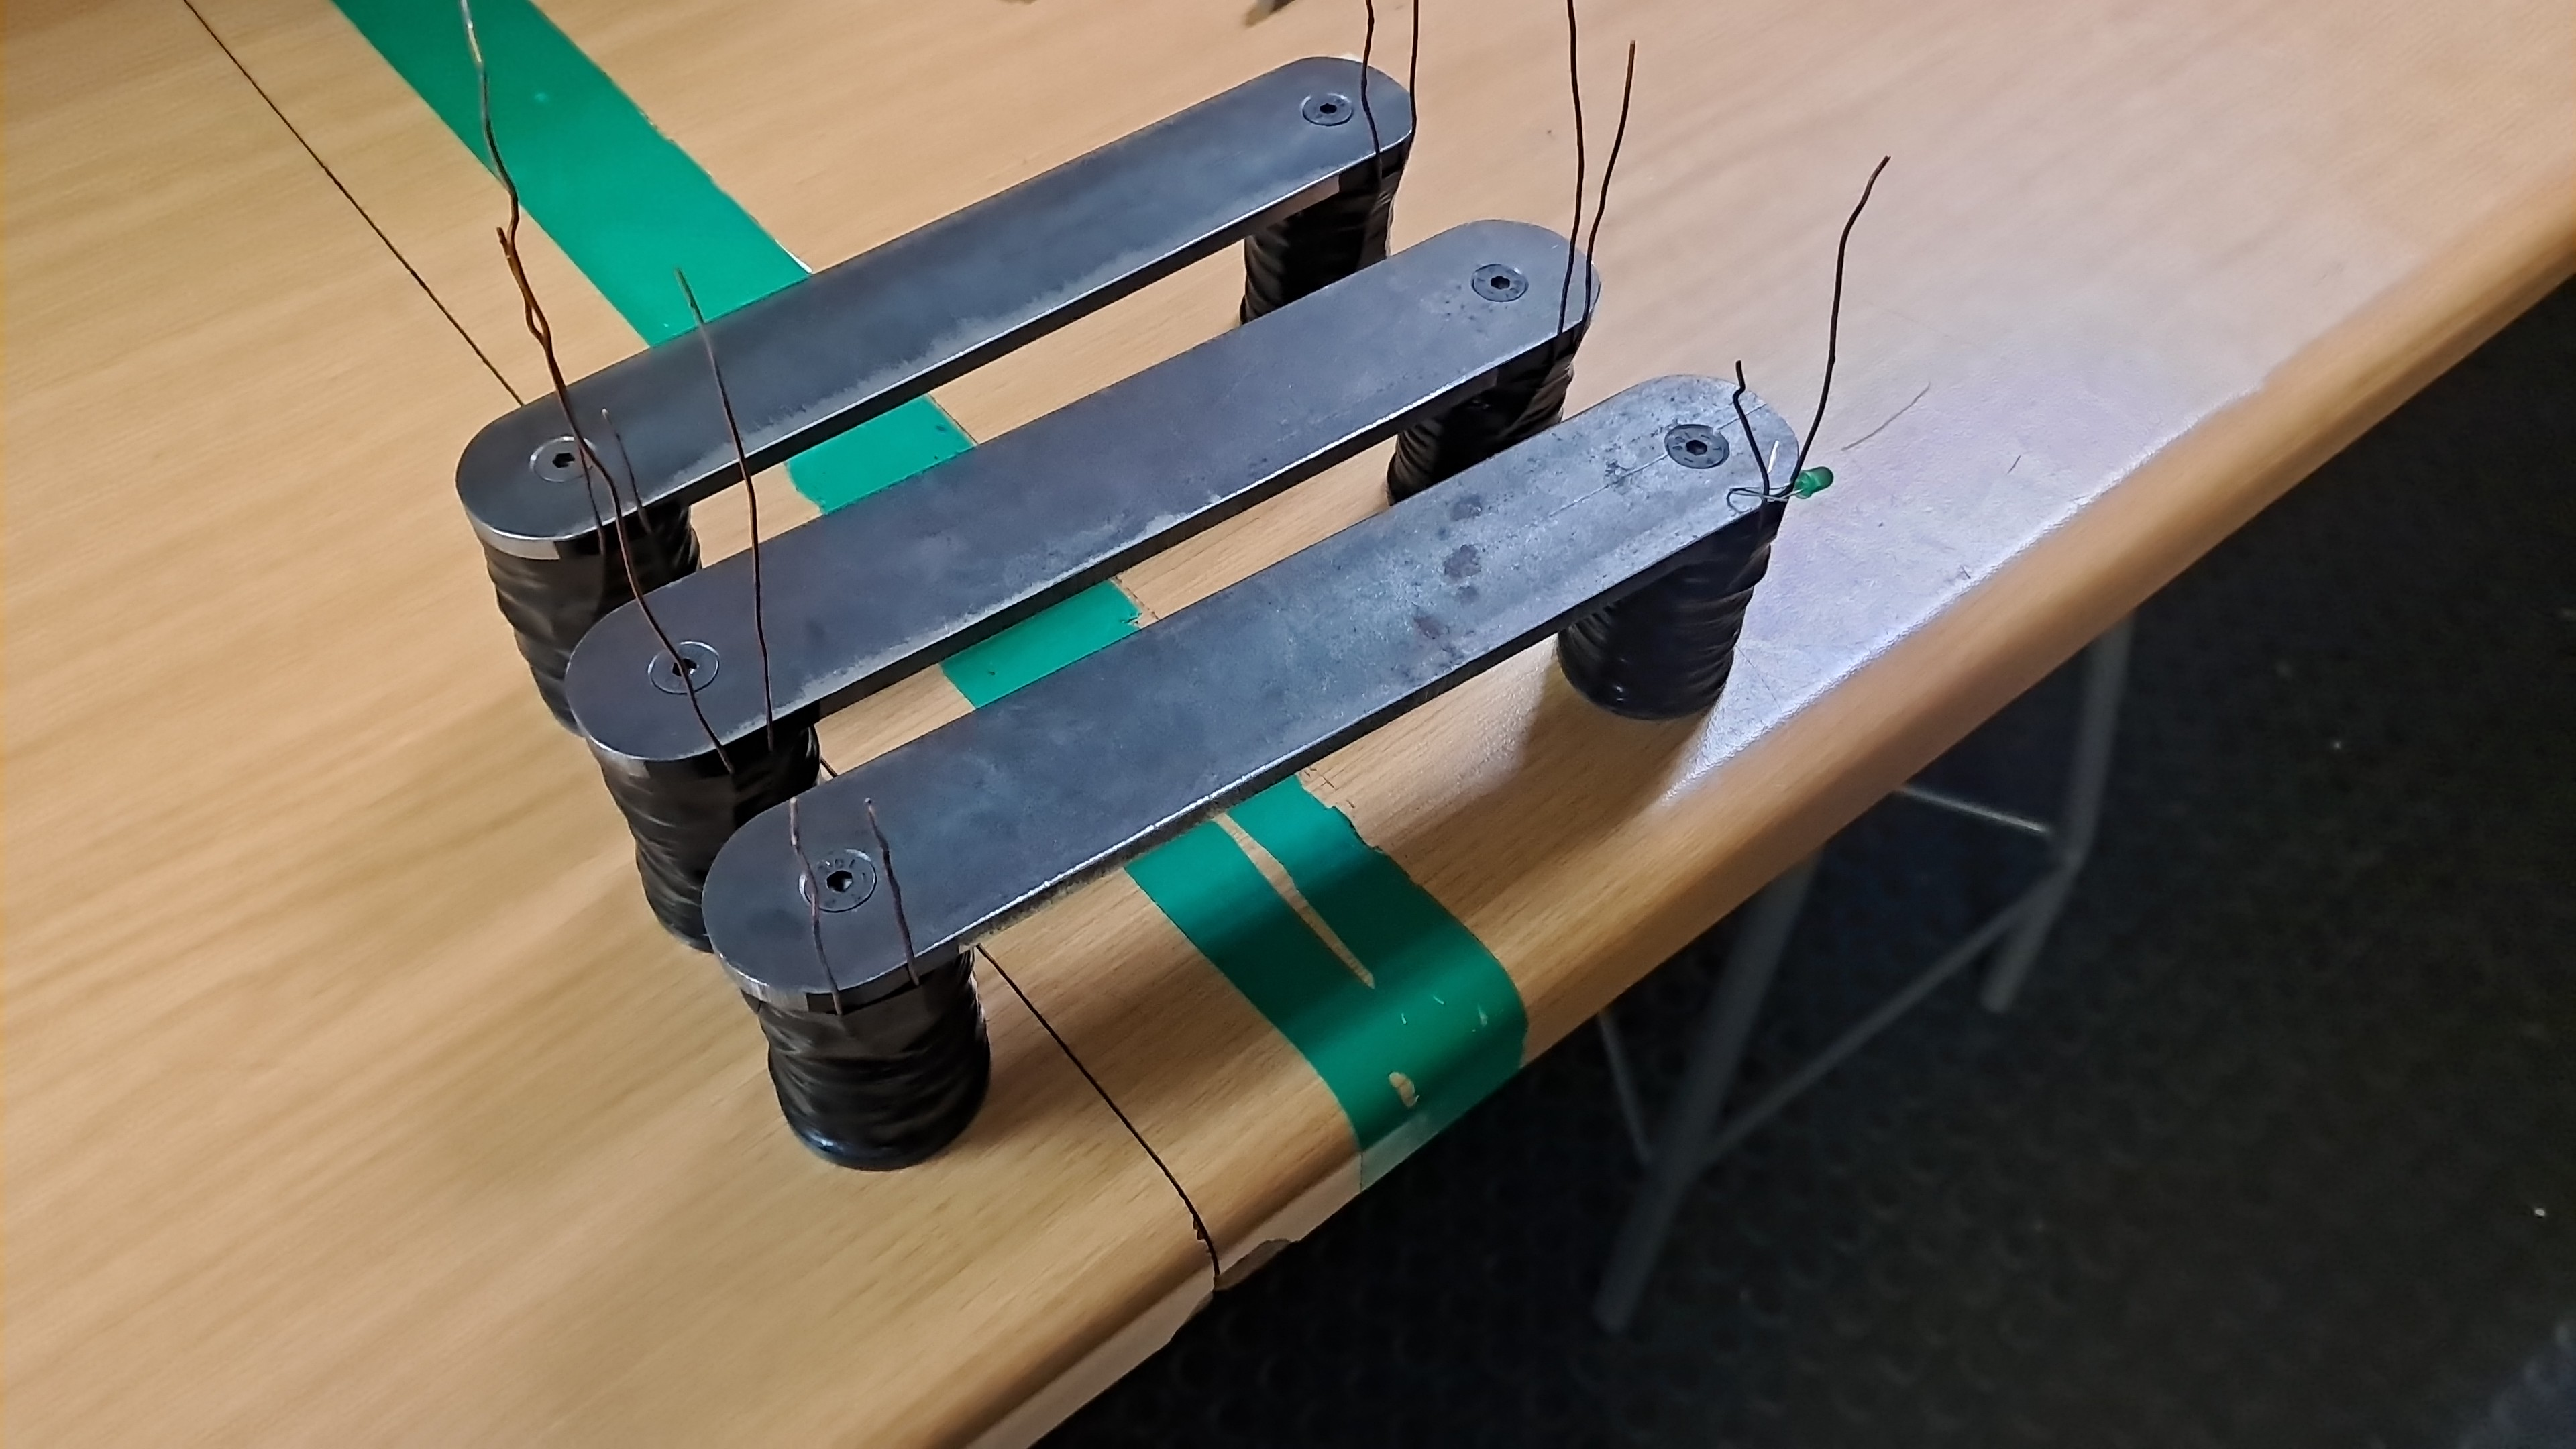
\includegraphics[width=0.95\textwidth]{figures/Magnets.jpeg}
    \caption{Physical U-core magnets}
    \label{fig:eeri2-magnet}
\end{figure}

\subsection{Power Switching and Gate Driver}
\label{subsec:eeri2-dec-driver}
The series coils have a high inductance ($L \approx 0.1\,\text{H}$ on-load) carrying $3\,\text{A}$ at $13.5\,\text{V}$.
De energising the magnet releases stored energy, causing high voltage spikes. Table~\ref{tab:eeri2-switching-tradeoff} evaluates three candidate switching technologies.

\begin{table}[H]
    \centering
    \small
    \caption{Trade-off evaluation of switching architectures.}
    \label{tab:eeri2-switching-tradeoff}
    \begin{tabularx}{\textwidth}{@{} >{\raggedright\arraybackslash}X *{5}{c} c c @{}}
        \toprule
        \textbf{Switching Architecture} & \textbf{Efficiency} & \textbf{Speed} & \textbf{Clamping} & \textbf{Life/PWM} & \textbf{Cost} & \textbf{Score} & \textbf{Selected} \\
        \textit{Criteria weighting} & \textit{0.30} & \textit{0.25} & \textit{0.20} & \textit{0.15} & \textit{0.10} & \textit{(1--5)} & \\
        \midrule
        Electromechanical relay (12\,V / 10\,A) & 4 & 1 & 2 & 1 & 5 & 2.50 & \\
        BJT (TIP120 + 1N4007)        & 2 & 2 & 2 & 3 & 4 & 2.35 & \\
        Power MOSFET (IRF540Z + TC4420 + MBR1060) & 5 & 5 & 5 & 5 & 4 & 4.90 & \checkmark \\
        \bottomrule
    \end{tabularx}
\end{table}

Electromechanical relays can arc, the contacts bounce, and it wears,
and are bad at PWM or fast emergency response.
A BJT (TIP120) exhibits a saturation voltage of 1.6, dissipating a lot of heat at $3,\text{A}$.
And the 1N4007 diode has a slow reverse recovery time ($> 2\,\mu\text{s}$) that may cause the transistor to be exposed to mutch voltage.

The combination of an IRF540Z N-channel MOSFET,
a TC4420 6\,A gate driver IC,
and an MBR1060 Schottky diode was selected.
The IRF540Z features an on-resistance of $27\,\text{m}\Omega$, this causes low conduction losses:
The TC4420 driver can source and sink up to $6\,\text{A}$ peak current directly from the $+13.5\,\text{V}$ rail, charging the gate capacitance ($C_{\mathrm{iss}} \approx 1000\,\text{pF}$) in $<25\,\text{ns}$.
This causes very low switching losses.
The MBR1060 Schottky diode ($60\,\text{V}$, $10\,\text{A}$) provides a current path across the coils.
This keeps the voltage over the switch well below the MOSFET rating ($V_{\mathrm{DSS}} = 100\,\text{V}$).

\section{MCTR I: Subsystem: Lateral Movement}
\label{sec:mctr1-subsystem-lateral-movement}

[Discuss the criteria for selecting this component (resolution,
power, size, cost, etc.). Present the options in a comparison
table.]

\begin{table}[H]
    \centering
    \caption{Available [Subsystem 1] options.}
    \label{tab:mctr1-options}
    \begin{tabular}{@{} l c c c c @{}}
        \toprule
        \textbf{Component} & \textbf{Criterion A} & \textbf{Criterion B}
            & \textbf{Criterion C} & \textbf{Selected} \\
        \midrule
        Option 1 & & & & \\
        Option 2 & & & & \checkmark \\
        Option 3 & & & & \\
        \bottomrule
    \end{tabular}
\end{table}

[Justify the selected option in one or two paragraphs.]

\begin{figure}[H]
    \centering
    %\includegraphics[width=0.40\textwidth]{subsystem1_photo}
    \caption{Selected [Subsystem 1] component.}
    \label{fig:mctr1-subsystem}
\end{figure}

\section{MCTR II: Subsystem: Spooling}
\label{sec:mctr2-subsystem-spooling}
% =====================================================================
%  mctr2_parameters.tex  --  MCTR II (Spooling) parameter + calculation sheet
%
%  HOW TO USE
%   * Edit ONLY the \In... values in Section 1. Everything in Section 2
%     (\Raw... results) is computed from them by \fpeval, so every
%     table, equation and sentence that quotes a result updates on the
%     next compile.
%   * Units are noted per line. Torques in N.m unless stated.
%   * Display helpers:  \shown{Name}{digits}        -> number only
%                       \showv{Name}{digits}{unit}  -> number + unit
%   * This file is safe to \input from several chapters (loads once).
%   * Needs: LaTeX >= 2021 (\fpeval in kernel), amsmath, xcolor.
% =====================================================================
\ifdefined\MCTRIIparamsloaded\else
\def\MCTRIIparamsloaded{}

\providecommand{\tbd}[1]{\textcolor{red}{\textbf{[TBD: #1]}}}
\newcommand{\val}[2]{\ensuremath{#1\,\mathrm{#2}}}
\newcommand{\shown}[2]{\fpeval{round(\csname Raw#1\endcsname,#2)}}
\newcommand{\showv}[3]{\val{\fpeval{round(\csname Raw#1\endcsname,#2)}}{#3}}
% PASS/FAIL helpers: \passge{value}{limit} passes when value >= limit
\newcommand{\passge}[2]{\ifdim #1pt<#2pt \textcolor{red}{\textbf{FAIL}}\else\textcolor{green!45!black}{\textbf{PASS}}\fi}
\newcommand{\passle}[2]{\ifdim #1pt>#2pt \textcolor{red}{\textbf{FAIL}}\else\textcolor{green!45!black}{\textbf{PASS}}\fi}

% Functional-unit number of MCTR II (Level 1 drawing: F/U 1.4).
% NOTE: the Level 2 drawing currently labels sub-units 1.3.x; change the
% drawing to 1.4.x (or set this to 1.3 to match the drawing, but 1.3 is MCTR I).
\newcommand{\fuMII}{1.3}

% ---------------------------------------------------------------------
% 1. INPUTS  (edit these)
% ---------------------------------------------------------------------
% -- Loads, stroke, timing
\newcommand{\InMassRated}{20}    % kg   rated payload (PHY1)
\newcommand{\InMassDesign}{30}   % kg   design overload case (analysis only)
\newcommand{\InMassAttach}{2}    % kg   magnet + hook hanging on rope  [TBD: weigh]
\newcommand{\InGrav}{9.81}       % m/s^2
\newcommand{\InStroke}{1.6}      % m     hoist stroke (PT2)
\newcommand{\InTimeReq}{20}      % s     max stroke time (PT2)
\newcommand{\InServiceF}{1.5}    % -     service factor on drum torque
\newcommand{\InSFreq}{1.5}       % -     minimum acceptable safety factor (strength checks)
% -- Drum and rope
\newcommand{\InDrumD}{50}        % mm    drum core diameter (FROZEN; 70 mm entry removed)
\newcommand{\InDrumH}{60}        % mm    drum usable length
\newcommand{\InRopeD}{5}         % mm    rope diameter
\newcommand{\InRopeCentre}{1}    % 1 = tension acts at rope centre-line (D+d); 0 = old spreadsheet (D only)
% -- Motor and VSD
\newcommand{\InMotorP}{180}      % W     Askari MS632-4
\newcommand{\InMotorN}{1360}     % rpm   at rated frequency
\newcommand{\InMotorF}{50}       % Hz    rated frequency
\newcommand{\InVsdF}{50}         % Hz    frequency VSD will actually deliver  [TBD: EEII I to confirm]
% -- Gearbox (stage A = motor side, stage B = drum side)
\newcommand{\InNpA}{16}   \newcommand{\InNgA}{102}   % pinion / gear teeth, stage A
\newcommand{\InNpB}{16}   \newcommand{\InNgB}{102}   % pinion / gear teeth, stage B
\newcommand{\InModA}{1.5} \newcommand{\InModB}{2}    % mm module
\newcommand{\InFwA}{10}   \newcommand{\InFwB}{15}    % mm face width
\newcommand{\InPhi}{25}          % deg   pressure angle (use 24 if Inventor forces it; both gears of a mesh must match)
\newcommand{\InYpA}{0.296}       % Lewis form factor, pinion  (Shigley Tbl 14-2, 20 deg value: conservative for 25 deg)
\newcommand{\InYgA}{0.447}       % Lewis form factor, gear
\newcommand{\InYpB}{0.296}
\newcommand{\InYgB}{0.447}
\newcommand{\InEta}{0.95}        % -     efficiency per gear stage
\newcommand{\InSigAllow}{20}     % MPa   allowable PETG root stress [GUESS: replace with printed-coupon result / SF]
\newcommand{\InClear}{0.25}      % mm    added centre-distance clearance (printed backlash)
\newcommand{\InBed}{220}         % mm    print bed edge length [TBD: confirm printer]
% -- Shaft, hub and fastener
\newcommand{\InShaftD}{10}       % mm    shaft diameter
\newcommand{\InSpan}{100}        % mm    bearing span (centre-to-centre)
\newcommand{\InKt}{2}            % -     bending stress-concentration factor, cross-hole
\newcommand{\InKts}{2}           % -     torsion stress-concentration factor, cross-hole
\newcommand{\InSy}{250}          % MPa   yield strength  [TBD: replace with certified grade, e.g. EN8 bright bar]
\newcommand{\InBoltD}{4}         % mm    cross-bolt diameter
\newcommand{\InHubWall}{8}       % mm    hub wall length bearing on bolt
\newcommand{\InHubAllow}{20}     % MPa   allowable PETG bearing stress [GUESS]
% -- Brake
\newcommand{\InBrakeSF}{2}       % -     brake torque safety factor
\newcommand{\InBrakeRated}{0}    % N.m   datasheet holding torque; 0 = not yet known  [TBD: datasheet]
% -- Load cell and HX711
\newcommand{\InCellCap}{100}     % kg    YZC-516 rated capacity
\newcommand{\InCellSens}{2}      % mV/V  rated output [TBD: datasheet]
\newcommand{\InExc}{5}           % V     excitation (HX711 supply)
\newcommand{\InGain}{128}        % -     HX711 channel A gain
\newcommand{\InSps}{80}          % SPS   HX711 output rate (RATE pin high)
\newcommand{\InFilt}{4}          % -     samples averaged by interlock filter
\newcommand{\InNoise}{500}       % counts peak-to-peak noise [GUESS: measure with motor running]
\newcommand{\InTrip}{1.25}       % -     overload trip as multiple of (rated + attachment)
% -- Cost (R, incl. VAT and shipping, from Cost_and_Budget.xlsx)
\newcommand{\InBudget}{5000}
\newcommand{\InCostBearings}{116.24}
\newcommand{\InCostCell}{429.00}     % [CHECK: sheet unit 493.35 + 135.70 shipping = 629.05]
\newcommand{\InCostHX}{179.40}       % [CHECK: unit price 43.70]
\newcommand{\InCostPSU}{390.17}
\newcommand{\InCostBrake}{907.68}    % excluded from the sheet's own subtotal

% ---------------------------------------------------------------------
% 2. DERIVED RESULTS  (do not edit)
% ---------------------------------------------------------------------
% -- Kinematics
\newcommand{\RawDeff}{\fpeval{\InDrumD+\InRopeCentre*\InRopeD}}
\newcommand{\RawVreq}{\fpeval{\InStroke*1000/\InTimeReq}}
\newcommand{\RawWraps}{\fpeval{\InStroke*1000/(pi*\RawDeff)}}
\newcommand{\RawWrapsFit}{\fpeval{floor(\InDrumH/\InRopeD)}}
\newcommand{\RawiA}{\fpeval{\InNgA/\InNpA}}
\newcommand{\RawiB}{\fpeval{\InNgB/\InNpB}}
\newcommand{\RawiT}{\fpeval{\RawiA*\RawiB}}
\newcommand{\RawNmot}{\fpeval{\InMotorN*\InVsdF/\InMotorF}}
\newcommand{\RawNdrum}{\fpeval{\RawNmot/\RawiT}}
\newcommand{\RawVline}{\fpeval{pi*\RawDeff*\RawNdrum/60}}
\newcommand{\RawTstroke}{\fpeval{\InStroke*1000/\RawVline}}
\newcommand{\RawSpeedMargin}{\fpeval{(\RawVline/\RawVreq-1)*100}}
\newcommand{\RawiReq}{\fpeval{pi*\RawDeff*\RawNmot/(60*\RawVreq)}}
\newcommand{\RawFmin}{\fpeval{\RawVreq*60*\RawiT/(pi*\RawDeff)*\InMotorF/\InMotorN}}
% -- Drum torque, motor sizing
\newcommand{\RawFropeR}{\fpeval{\InMassRated*\InGrav}}
\newcommand{\RawFropeD}{\fpeval{\InMassDesign*\InGrav}}
\newcommand{\RawTdrR}{\fpeval{\InMassRated*\InGrav*\RawDeff/2000}}
\newcommand{\RawTdrD}{\fpeval{\InMassDesign*\InGrav*\RawDeff/2000*\InServiceF}}
\newcommand{\RawTdrSheet}{\fpeval{\InMassDesign*\InGrav*\InDrumD/2000*\InServiceF}}
\newcommand{\RawEtaGB}{\fpeval{\InEta*\InEta}}
\newcommand{\RawTmReq}{\fpeval{\RawTdrR/(\RawiT*\RawEtaGB)}}
\newcommand{\RawTmRated}{\fpeval{\InMotorP/(2*pi*\InMotorN/60)}}
\newcommand{\RawTmMargin}{\fpeval{\RawTmRated/\RawTmReq}}
\newcommand{\RawPmech}{\fpeval{\InMassRated*\InGrav*\RawVline/1000/\RawEtaGB}}
\newcommand{\RawPavail}{\fpeval{\InMotorP*\InVsdF/\InMotorF}}
% -- Gear loads (design case) and Lewis stress
\newcommand{\RawTtwo}{\fpeval{\RawTdrD/(\RawiB*\InEta)}}
\newcommand{\RawTone}{\fpeval{\RawTtwo/(\RawiA*\InEta)}}
\newcommand{\RawFtB}{\fpeval{2*\RawTtwo*1000/(\InModB*\InNpB)}}
\newcommand{\RawFtA}{\fpeval{2*\RawTone*1000/(\InModA*\InNpA)}}
\newcommand{\RawFnB}{\fpeval{\RawFtB/cosd(\InPhi)}}
\newcommand{\RawFnA}{\fpeval{\RawFtA/cosd(\InPhi)}}
\newcommand{\RawFrB}{\fpeval{\RawFtB*tand(\InPhi)}}
\newcommand{\RawSigPA}{\fpeval{\RawFtA/(\InFwA*\InModA*\InYpA)}}
\newcommand{\RawSigGA}{\fpeval{\RawFtA/(\InFwA*\InModA*\InYgA)}}
\newcommand{\RawSigPB}{\fpeval{\RawFtB/(\InFwB*\InModB*\InYpB)}}
\newcommand{\RawSigGB}{\fpeval{\RawFtB/(\InFwB*\InModB*\InYgB)}}
\newcommand{\RawSFpA}{\fpeval{\InSigAllow/\RawSigPA}}
\newcommand{\RawSFpB}{\fpeval{\InSigAllow/\RawSigPB}}
% -- Gear geometry
\newcommand{\RawDpinA}{\fpeval{\InModA*\InNpA}}
\newcommand{\RawDgearA}{\fpeval{\InModA*\InNgA}}
\newcommand{\RawDpinB}{\fpeval{\InModB*\InNpB}}
\newcommand{\RawDgearB}{\fpeval{\InModB*\InNgB}}
\newcommand{\RawDoGearA}{\fpeval{\InModA*(\InNgA+2)}}
\newcommand{\RawDoGearB}{\fpeval{\InModB*(\InNgB+2)}}
\newcommand{\RawCdA}{\fpeval{\InModA*(\InNpA+\InNgA)/2+\InClear}}
\newcommand{\RawCdB}{\fpeval{\InModB*(\InNpB+\InNgB)/2+\InClear}}
\newcommand{\RawZmin}{\fpeval{2/(sind(\InPhi)^2)}}
\newcommand{\RawDbPinB}{\fpeval{\RawDpinB*cosd(\InPhi)}}
\newcommand{\RawBedUse}{\fpeval{max(\RawDoGearA,\RawDoGearB)/\InBed*100}}
% -- Shaft (macros with arguments: #1 = payload mass kg, #2 = torque factor)
\newcommand{\Tdr}[2]{\fpeval{#1*\InGrav*\RawDeff/2*#2}}                                   % N.mm
\newcommand{\FgB}[2]{\fpeval{2*\Tdr{#1}{#2}/(\InEta*\InModB*\InNgB*cosd(\InPhi))}}        % N
\newcommand{\Msh}[2]{\fpeval{(#1*\InGrav+\FgB{#1}{#2})*\InSpan/4}}                        % N.mm
\newcommand{\SigBsh}[2]{\fpeval{32*\Msh{#1}{#2}/(pi*\InShaftD^3)}}                        % MPa
\newcommand{\Taush}[2]{\fpeval{16*\Tdr{#1}{#2}/(pi*\InShaftD^3)}}                         % MPa
\newcommand{\VMsh}[2]{\fpeval{sqrt((\InKt*\SigBsh{#1}{#2})^2+3*(\InKts*\Taush{#1}{#2})^2)}} % MPa
\newcommand{\RawFgD}{\FgB{\InMassDesign}{\InServiceF}}
\newcommand{\RawMshD}{\Msh{\InMassDesign}{\InServiceF}}
\newcommand{\RawSigBD}{\SigBsh{\InMassDesign}{\InServiceF}}
\newcommand{\RawTauD}{\Taush{\InMassDesign}{\InServiceF}}
\newcommand{\RawVMD}{\VMsh{\InMassDesign}{\InServiceF}}
\newcommand{\RawVMR}{\VMsh{\InMassRated}{1}}
\newcommand{\RawSFsD}{\fpeval{\InSy/\RawVMD}}
\newcommand{\RawSFsR}{\fpeval{\InSy/\RawVMR}}
% -- Hub / cross-bolt (design case, drum shaft)
\newcommand{\RawFside}{\fpeval{\RawTdrD*1000/\InShaftD}}
\newcommand{\RawSigHub}{\fpeval{\RawFside/(\InBoltD*\InHubWall)}}
\newcommand{\RawTauBolt}{\fpeval{\RawFside/(pi*\InBoltD^2/4)}}
\newcommand{\RawSFhub}{\fpeval{\InHubAllow/\RawSigHub}}
% -- Rated-case (20 kg, no service factor) checks for gears and hub
\newcommand{\RawLoadRatio}{\fpeval{\RawTdrR/\RawTdrD}}
\newcommand{\RawSFpAR}{\fpeval{\RawSFpA/\RawLoadRatio}}
\newcommand{\RawSFpBR}{\fpeval{\RawSFpB/\RawLoadRatio}}
\newcommand{\RawSigHubR}{\fpeval{\RawSigHub*\RawLoadRatio}}
\newcommand{\RawSFhubR}{\fpeval{\InHubAllow/\RawSigHubR}}
% -- Brake
\newcommand{\RawTholdDrum}{\fpeval{\InMassDesign*\InGrav*\RawDeff/2000}}
\newcommand{\RawTholdIn}{\fpeval{\RawTholdDrum/\RawiT}}
\newcommand{\RawBrakeReqDrum}{\fpeval{\RawTholdDrum*\InBrakeSF}}
\newcommand{\RawBrakeReqIn}{\fpeval{\RawTholdIn*\InBrakeSF}}
\newcommand{\BrakeMarginIn}{\ifdim\InBrakeRated pt=0pt\tbd{datasheet torque}\else\fpeval{round(\InBrakeRated/\RawBrakeReqIn,1)}\fi}
\newcommand{\BrakeMarginDrum}{\ifdim\InBrakeRated pt=0pt\tbd{datasheet torque}\else\fpeval{round(\InBrakeRated/\RawBrakeReqDrum,1)}\fi}
% -- Load cell and HX711
\newcommand{\RawFcell}{\fpeval{(\InMassRated+\InMassAttach)*\InGrav}}
\newcommand{\RawMtrip}{\fpeval{(\InMassRated+\InMassAttach)*\InTrip}}
\newcommand{\RawCellUse}{\fpeval{\RawMtrip/\InCellCap*100}}
\newcommand{\RawSigFS}{\fpeval{\InCellSens*\InExc}}
\newcommand{\RawAdcRange}{\fpeval{0.5*\InExc/\InGain*1000}}
\newcommand{\RawCntPerKg}{\fpeval{\InCellSens/1000/\InCellCap*\InGain/0.5*2^23}}
\newcommand{\RawResG}{\fpeval{\InNoise/\RawCntPerKg*1000}}
\newcommand{\RawLatency}{\fpeval{\InFilt/\InSps*1000}}
\newcommand{\RawTravel}{\fpeval{\RawVline*\RawLatency/1000}}
% -- Cost
\newcommand{\RawCostTot}{\fpeval{\InCostBearings+\InCostCell+\InCostHX+\InCostPSU+\InCostBrake}}
\newcommand{\RawBudgetLeft}{\fpeval{\InBudget-\RawCostTot}}
\newcommand{\RawBudgetUse}{\fpeval{\RawCostTot/\InBudget*100}}
\fi


The spooling subsystem was selected against five criteria: \textbf{fail-safe
behaviour} (the load must be held when power or command is lost, FR6),
\textbf{compliance} with the design requirements (no worm gear, DR2; minimum
two stages), \textbf{cost} within the R\InBudget{} group cap, \textbf{manufacturability}
with the workshop tools available (3D printing, drill press), and
\textbf{verifiability} by the tests in Chapter~\ref{ch:test-plan}. All strength
figures below are produced by the parameter sheet in Appendix~\ref{app:technical};
changing an input there updates every number quoted here.
 
\subsection{Holding brake type}
\begin{table}[H]
    \centering
    \caption{Available holding-brake options for MCTR II.}
    \label{tab:mctr2-brake-type}
    \small
    \begin{tabular}{@{} l c c c c c @{}}
        \toprule
        \textbf{Option} & \textbf{Fail-safe} & \textbf{Bidirectional} & \textbf{DR2 ok}
            & \textbf{Cost} & \textbf{Selected} \\
        \midrule
        One-way (sprag) clutch            & No  & No  & Yes & Low  & \\
        Self-locking worm gear            & Yes & Yes & No  & Low  & \\
        VSD / DC-injection braking only   & No  & Yes & Yes & None & \\
        Spring-applied, electrically released brake & Yes & Yes & Yes & Medium & \checkmark \\
        \bottomrule
    \end{tabular}
\end{table}
A one-way clutch locks in one direction only, so it cannot permit powered
lowering and has no engaged or released state to monitor. A worm gear is
prohibited by DR2. Electrical braking disappears with the power it relies on.
A spring-applied brake that is released by energising its coil engages when
power is lost, which is exactly the behaviour FR6 requires.
 
\subsection{Brake source and mounting position}
A trolley drive-motor brake assembly (R\InCostBrake{} including shipping) was
chosen because the next commercially available option cost about R5\,000,
which alone would exhaust the project budget. It is released by a separate
48\,V supply.
\begin{table}[H]
    \centering
    \caption{Brake mounting position options.}
    \label{tab:mctr2-brake-pos}
    \small
    \begin{tabular}{@{} l c p{5.2cm} c @{}}
        \toprule
        \textbf{Position} & \textbf{Torque to hold} & \textbf{Protects against} & \textbf{Selected} \\
        \midrule
        Motor shaft & $<$ input value & Motor loss only; fan side not free & \\
        Gearbox input stub shaft & \showv{BrakeReqIn}{2}{N\,m} & Motor, coupling and stage~A failure & \checkmark\ (provisional) \\
        Drum shaft & \showv{BrakeReqDrum}{1}{N\,m} & Everything including gear failure & \\
        \bottomrule
    \end{tabular}
\end{table}
The input stub shaft needs only a small holding torque, which suits a
low-cost brake. The residual risk is that a stripped stage~B tooth would
release the load, and this must be accepted explicitly or the brake moved to
the drum shaft. The datasheet holding torque, coil voltage and shaft bore of the
purchased brake are not yet verified: \tbd{enter in \texttt{\textbackslash InBrakeRated}; margin is currently
\BrakeMarginIn}.
 
\subsection{Gearbox configuration and gear material}
A two-stage compound spur gearbox in 3D-printed PETG was chosen. A single
stage would violate the two-stage minimum of the work-package scope and would need
a gear of unmanageable diameter, and a planetary train is too difficult to print
with the required accuracy. Stage A (motor side) uses module \InModA\,mm and stage B
(drum side) module \InModB\,mm: stage A is limited by what a printer can form, not
by strength, while stage B carries the load. The tooth counts are
$N_p=\InNpA$, $N_g=\InNgA$ per stage, giving an overall ratio of \shown{iT}{2}:1.
Pressure angle is \InPhi$^\circ$ for every gear (both gears of a mesh must share it).
The largest gear has an outside diameter of \showv{DoGearB}{0}{mm}, which uses
\shown{BedUse}{0}\% of the assumed \InBed\,mm print bed.
 
Lewis bending stress at the rated load gives a stage~B pinion safety factor
of \shown{SFpBR}{2} against the assumed allowable of \InSigAllow\,MPa. That allowable
is a guess until a printed test pair has been loaded to failure on the test rig;
the failure torque divided by the safety factor then replaces it.
The full workings are in Appendix~\ref{app:technical}.
 
\subsection{Shaft material and gear fastening}
\begin{table}[H]
    \centering
    \caption{Options for fastening gears and drum to the shafts.}
    \label{tab:mctr2-fastening}
    \small
    \begin{tabular}{@{} l c c c c @{}}
        \toprule
        \textbf{Option} & \textbf{Makeable in workshop} & \textbf{Stiffness}
            & \textbf{Stress raiser} & \textbf{Selected} \\
        \midrule
        Taper-lock bush                         & No (needs precise taper) & High & Low    & \\
        Flexible (spider) coupling between gear and shaft & Yes & Low (backlash) & Low & \\
        Keyway in shaft                          & Hard on 10\,mm bar       & High & High   & \\
        Hub with cross-bolt through reamed hole  & Yes (drill press + jig)  & High & Medium & \checkmark \\
        \bottomrule
    \end{tabular}
\end{table}
Each gear gets a printed hub through which a bolt passes into a hole drilled
through the shaft, retained by a nut. A flexible coupling between a gear and its shaft
would add torsional compliance exactly where holding stiffness matters, so
flexible couplings are used only between the motor and the gearbox.
 
The test rig failure was traced to poor shaft design: standard steel of unknown
grade, weakened by stress concentrations from poor milling and drilling. The
following measures answer that cause directly: certified bright bar of known grade,
holes drilled and reamed on a drill press with a jig and deburred, and no holes near shoulders.
The shaft check at the design overload (\InMassDesign\,kg with service factor
\InServiceF) gives a von Mises stress of \showv{VMD}{0}{MPa} and a safety factor of
\shown{SFsD}{2}, which \ifdim\RawSFsD pt<\InSFreq pt\textcolor{red}{\textbf{does not meet}}\else meets\fi\ the
required \InSFreq. At the rated payload the safety factor is \shown{SFsR}{2}.
If the check does not close with the certified grade, the drum shaft becomes 12\,mm
(only the coupling and bearing bores change).
 
\subsection{Motor-to-gearbox coupling}
\begin{table}[H]
    \centering
    \caption{Motor coupling options.}
    \label{tab:mctr2-coupling}
    \small
    \begin{tabular}{@{} l c c c @{}}
        \toprule
        \textbf{Option} & \textbf{Absorbs misalignment} & \textbf{Protects motor bearings} & \textbf{Selected} \\
        \midrule
        Rigid coupling                      & No  & Yes if stub on bearings & \\
        Pinion overhung on motor shaft      & No  & No (gear radial load)   & \\
        Flexible jaw/spider coupling to a separately supported stub shaft & Yes & Yes & \checkmark \\
        \bottomrule
    \end{tabular}
\end{table}
The motor shaft is 11\,mm with a $4\times16$\,mm keyway and the gearbox input shaft is
\InShaftD\,mm. A coupling sized for one shaft will be bored out for the other.
Torque at this interface is only \showv{TmReq}{2}{N\,m} against a motor rating of
\showv{TmRated}{2}{N\,m}.
 
\subsection{On-hook load measurement}
\begin{table}[H]
    \centering
    \caption{Load measurement options.}
    \label{tab:mctr2-loadcell}
    \small
    \begin{tabular}{@{} l c c c @{}}
        \toprule
        \textbf{Option} & \textbf{Cost} & \textbf{Interlock speed} & \textbf{Selected} \\
        \midrule
        ADS1220 24-bit SPI ADC & Not affordable locally & High (up to 2\,kSPS) & \\
        HX711 module           & About R48              & \InSps\,SPS when RATE pin high & \checkmark \\
        \bottomrule
    \end{tabular}
\end{table}
The HX711 is selected on cost. Many modules tie the rate pin low (10\,SPS); the
purchased board must be checked and modified for \InSps\,SPS. With a
\InFilt-sample filter the detection latency is \showv{Latency}{0}{ms}, during which the
rope moves \showv{Travel}{1}{mm} at full speed. A \InCellCap\,kg S-type cell is used,
operating at \shown{CellUse}{0}\% of capacity at the overload trip. The rope passes over
a sheave suspended from the cell rather than through a fixed hook or sleeve, whose
friction would corrupt the reading. The drum-side rope leg must be horizontal so that
only the payload weight acts along the cell axis.
 
\subsection{Bearings and base plate}
Eight 6000-2RS bearings (10\,mm bore) match the shaft size. A printed housing wall is
not to rely on interference alone: a shoulder and a bolted retaining plate hold each
bearing. The baseplate is 6061-T6 aluminium with machine-cut bearing bores.
 
\subsection{Assumptions and limitations}
\begin{itemize}
    \item The payload electromagnet fails safe (or not) under the responsibility of the
          engineer for EEII~II. The hoist brake holds the rope, not the payload attachment.
    \item The assembly exists for about five days and runs for about 30 minutes, so
          creep of PETG is not considered a governing mechanism.
    \item The 30\,kg case is an analysis margin; the rated payload is \InMassRated\,kg (PHY1).
    \item The motor may not reach \InMotorN\,rpm on the custom VSD. At \InVsdF\,Hz the stroke
          takes \showv{Tstroke}{1}{s}; the VSD must deliver at least \showv{Fmin}{1}{Hz} to meet
          the \InTimeReq\,s requirement.
\end{itemize}
 
\begin{figure}[H]
    \centering
    %\includegraphics[width=0.40\textwidth]{mctr2_selected}
    \caption{Selected MCTR II components (photograph to be added).}
    \label{fig:mctr2-selected}
\end{figure}

\section{REII: Subsystem: Remote Control Dashboard}
\label{sec:reii-subsystem-remote-control-dashboard}

The proposed design prioritises reliable command delivery,
dashboard responsiveness and local fault handling.
Earlier tests used two ESP32 boards and two 1000-packet trials
per condition, at distances up to 16~m.
Table~\ref{tab:reii-options} compares the radio configurations;
Appendix~C.3 records the trial counts.
\cite{reii_measurements2026}

\begin{table}[H]
    \centering
    \footnotesize
    \caption{Available radio configurations.}
    \label{tab:reii-options}

    \begin{tabularx}{\textwidth}{@{}
        >{\raggedright\arraybackslash}p{3.5cm}
        *{4}{>{\centering\arraybackslash}X}
    @{}}
        \toprule
        \textbf{Configuration} &
        \textbf{Loss at 8~m}\newline ACK off &
        \textbf{Loss at 16~m}\newline ACK on &
        \textbf{Reported Wi-Fi channel 1 overlap} &
        \textbf{Selected} \\
        \midrule

        Channel 76, 250~kbps &
        3.30\% & 0.00\% & No & Yes \\[3pt]

        Channel 76, 2~Mbps &
        4.40\% & 0.05\% & No & No \\[3pt]

        Channel 12, 250~kbps &
        16.10\% & Not tested & Yes & No \\[3pt]

        Channel 12, 2~Mbps &
        5.50\% & Not tested & Yes & No \\

        \bottomrule
    \end{tabularx}
\end{table}

\noindent
\textbf{Radio configuration.}
Channel 76 and 250~kbps are provisionally selected for lower
packet loss at longer tested distances, favouring reliable
delivery over nominal data rate. Channel 12 overlapped the
reported laboratory Wi-Fi allocation. Acknowledgements and
retries improved delivery in the earlier tests.
\cite{reii_measurements2026}
The runtime power setting of 2 and final ESP32-S3 response
times still require validation.

\noindent
\textbf{Communication and local control.}
Communication is handled separately from the dashboard
controls to keep the interface responsive while waiting
for replies. Messages have a fixed length of 32 bytes to
simplify processing. A radio acknowledgement confirms
message delivery; a separate controller reply indicates
whether the command was accepted. The ESP32-S3 would
generate control outputs and respond to communication
loss locally. The dashboard would calculate anti-sway
motion profiles and paths around known obstacles, which
the controller would execute through MCTR I's lateral
drive.
\cite{nwu_reii_scope2026}
These functions still require validation.

\noindent
\textbf{Starting reference.}
Marked upper-hoist parking with clearance and a marked
trolley position would provide a repeatable starting
condition. While stationary and disarmed, the operator
would select \emph{Confirm starting position} to set
the lateral reference before arming, without automatic
movement. Encoder feedback would then track lateral
position. This feature remains to be implemented.

\begin{figure}[H]
    \centering
    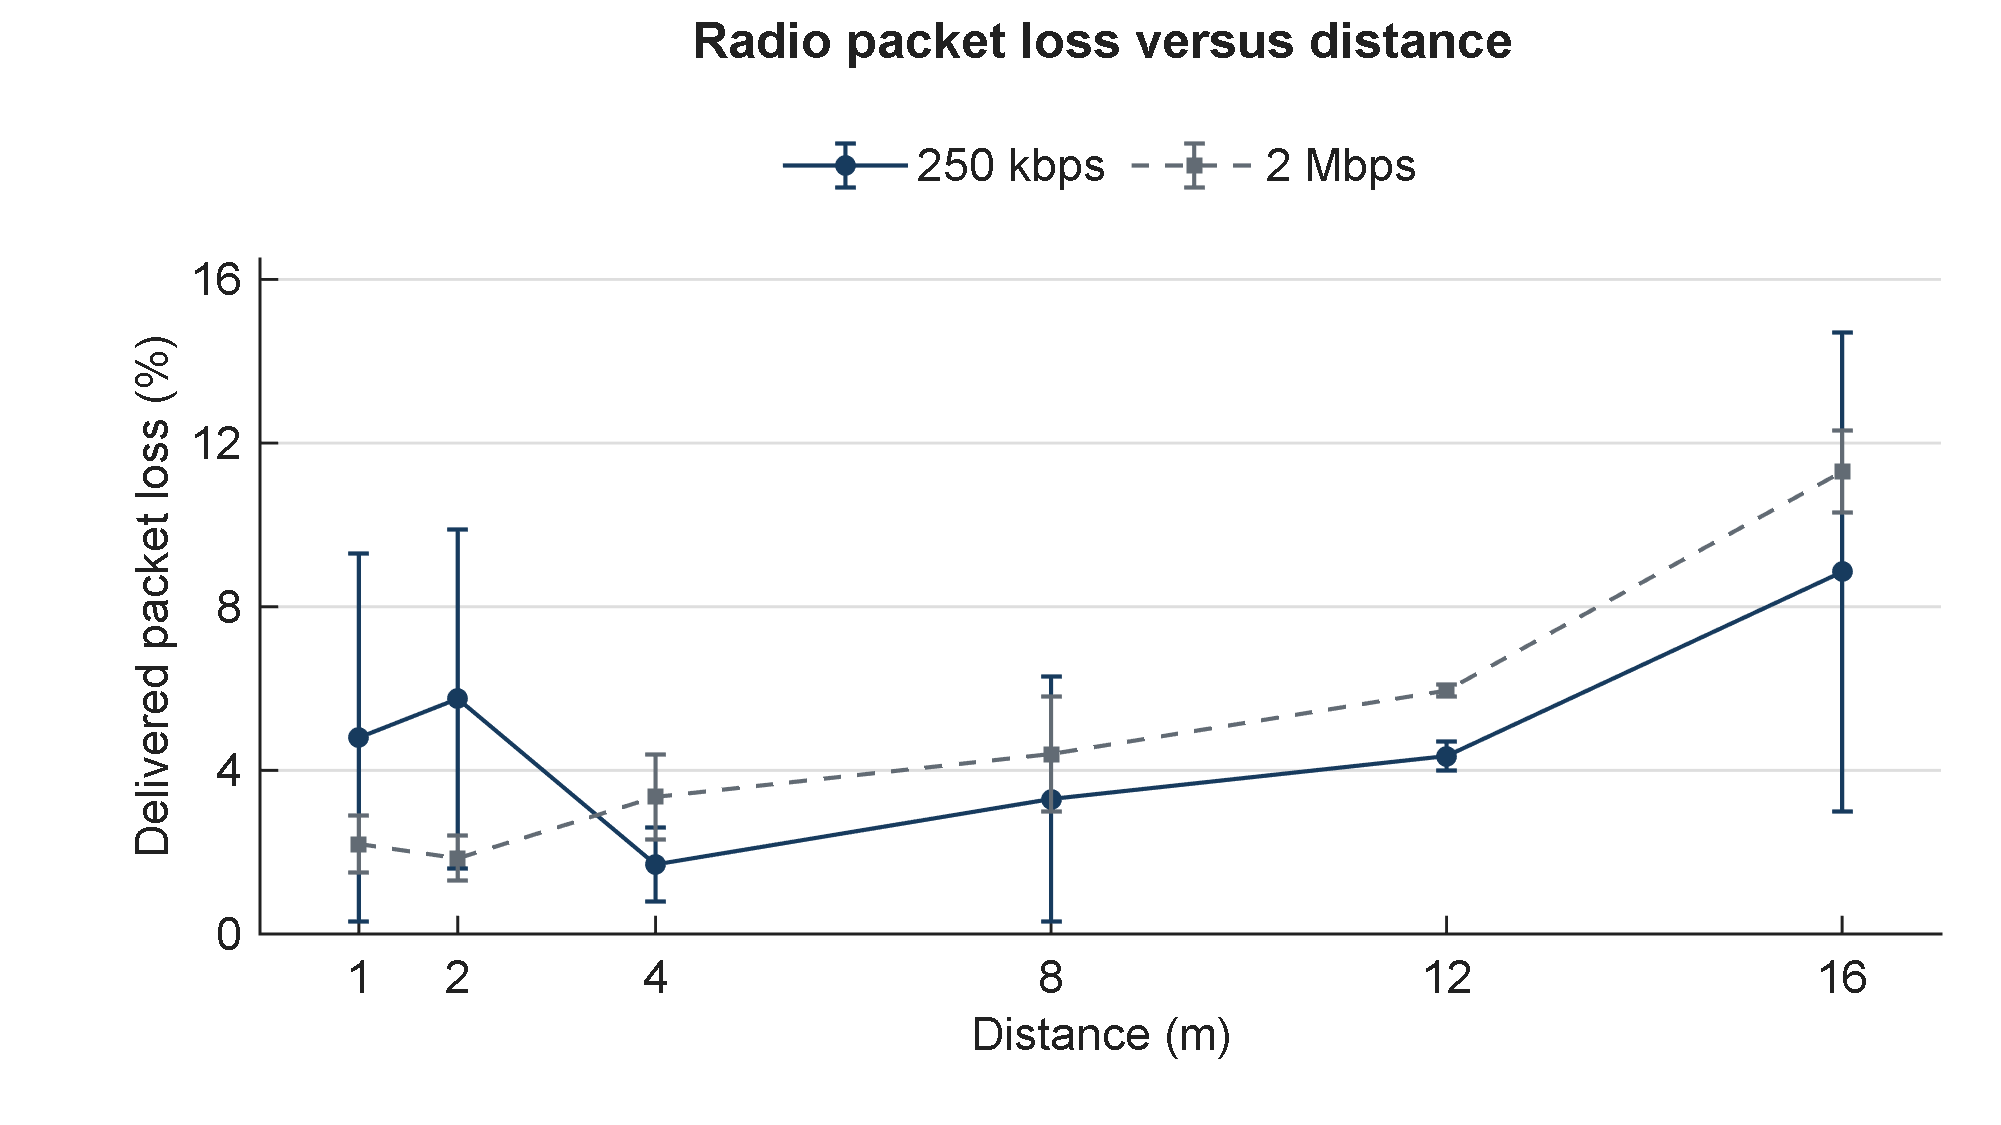
\includegraphics[width=0.80\textwidth]
        {figures/Figure_5_5_Radio_Performance.png}
    \caption{Radio packet loss versus distance on channel 76,
        supporting the provisional 250~kbps selection.
        Acknowledgements and retries were disabled.
        Points are means of two trials; bars show the
        two trial values.
        \cite{reii_measurements2026}}
    \label{fig:reii-subsystem}
\end{figure}